\chapter{周期含时驱动的光晶格系统} 
\label{chap:floq}
% \label{sec:chap4_floq}

在这一章中,我们来讨论周期含时驱动的光晶格体系。首先,我们在第 \ref{sec:floq:theory} 小节建立周期含时体系的 Floquet 理论,对 Floquet 理论进行相对完整、自洽的形式化表述;在 \ref{sec:floq:sl} 小节我们介绍在冷原子物理中周期含时驱动的一个例子——周期性晃动的光晶格,并推导出晃动光晶格在不同坐标系下的哈密顿量形式;在 \ref{sec:floq:heff} 小节,我们讨论一般的 Floquet 频闪有效静态模型,利用上一节的晃动光晶格的模型,我们推导出其相应的某一类频闪静态有效模型;在第 \ref{sec:floq:resona} 节,我们讨论一种特殊的情况——近共振的周期驱动,并讨论 Fermi Hubbard 单带模型的近共振驱动,推导出带有关联隧穿效应的 Fermi Hubbard 模型,该模型在 2018年 由苏黎世联邦理工学院的 Tilman Esslinger 教授领导的实验小组在蜂巢晶格中实现\cite{correlated-tunnel-expr-2018-shaking};在 \ref{sec:floqhubb} 小节中,我们讨论这种近共振周期驱动及其引发的关联隧穿效应所带来的物理后果,特别的,我们研究了在二维正方晶格上的情况,发现系统在小相互作用区域支持铁磁相和相分离\cite{floqhubb};我们采用了标准的路径积分方法做平均场处理,嵌套效应(Nesiting)的存在使得该方法在小相互作用的情况下合理可靠。


\section{周期含时体系的 Floquet 理论} \label{sec:floq:theory}
对于周期含时依赖的系统,Floquet 理论给出了一套形式描述\cite{floquet2017}。对周期含时系统有 $H(t+T) = H(t)$,$T$ 为时间周期。由于有时间方向的周期性存在,体系含时演化的本征态可以写成如下的 Floquet 态 
\begin{align}
\Psi_{\alpha}(t) &= e^{-\ii\varepsilon_{\alpha}t}\Phi_{\alpha}(t) \\
\Phi_{\alpha}(t) &= \Phi_{\alpha}(t+T)
\end{align}
这类似于固体物理中的 Bloch 定理,有空间周期性存在时本征态为如下形式的 Bloch 态
\begin{align}
\psi_{\alpha}(\vec{r}) &= e^{\ii\vec{r}\cdot\vec{a}}\phi_{\alpha}(\vec{r}) \\
\phi_{\alpha}(\vec{r}) &= \phi_{\alpha}(\vec{r}+\vec{a})
\end{align}
以上两者均可由群论证明。
\footnote{一个简单的理解方式是,由于体系有时间方向或空间方向的离散平移对称性,而平移群为阿贝尔群,而阿贝尔群的所有不可约表示都是一维表示,而量子力学需要的是幺正表示,那么对于空间平移算符 $e^{i\hat{p}a}$ 和周期时间演化算符 $U(t, t+T)$ ,其幺正表示就是简单的 $e^{i\theta}$ 。}
下面给出 Floquet 情况的证明。
\begin{proof}
周期幺正演化算符为
\begin{align}
U_F(t,t+T) = \mathcal{T} e^{-\ii\int_t^{t+T}H(t')dt'}
\end{align}
体系在时间方向的离散平移对称性决定满足薛定谔方程的本征态可以为以上算符的本征态,我们来显式地验证:
\begin{align}
\partial_tU_F &= -\ii[H(t+T)U_F - U_FH(t)] \\
&= -\ii[H(t)U_F - U_FH(t)]
\end{align}
这里用到了 $H(t) = H(t+T)$ 的周期性条件。因此,
\begin{align}
[\ii\partial_t - H, U_F] = 0
\end{align}
证毕。
\end{proof}

$\varepsilon_{\alpha}$ 称为准能量。不同准能量的 Floquet 态是正交的,证明如下:
\begin{align}
\langle \alpha|\beta \rangle &= \langle \alpha|U^{\dagger}(T)|U(T)|\beta \rangle \\
&= e^{-\ii(\varepsilon_{\alpha}-\varepsilon_{\beta})T}\langle \alpha|\beta \rangle \\
\therefore \langle \alpha|\beta \rangle &= 0
\end{align}

我们将上述形式的 $\Psi_{\alpha}(t)$ 带入薛定谔方程,有
\begin{align}
(H(t) - \ii\partial_t) \Psi_{\alpha}(t) = 0
\end{align}
由上式可得
\begin{align}
(H(t) - \ii\partial_t) \Phi_{\alpha}(t) = \varepsilon_{\alpha} \Phi_{\alpha}(t)
\end{align}
可见 $\Phi_{\alpha}(t)$ 满足 $H(t) - \ii\partial_t$ 的本征方程。
我们引入 Floquet 哈密顿量 $H_F$ 来标记这个算符, 
\begin{align}
H_F(t) = H(t) - \ii\partial_t
\end{align}
并称 $\Phi(t)$ 为 Floquet 模式,则 Floquet 模式是 $H_F$ 的本征模式。准能量可以取在 $\omega = 2\pi/T$ 的周期内,例如 $\varepsilon_{\alpha}\in[0,\omega)$,$\omega$ 是系统周期性时间依赖的频率。若能量超出这个范围,可以通过模掉整数个 $\omega$ 来折叠到这个范围内,类似于固体物理中模掉整数个倒格矢折叠进第一布里渊区。引入一个新的量子数 $m$ 来标记,即 $\Phi_{\alpha}^{m}(t)=e^{\ii m\omega t}\Phi_{\alpha}(t)$,则$\{\Phi_{\alpha}^{m}\}$ 构成 Floquet 哈密顿量希尔伯特空间的一组正交完备基,
\begin{align}
\langle\langle \Phi_{\alpha}^{m}|\Phi_{\beta}^{n}\rangle\rangle
= \dfrac{1}{T}\int_0^T \langle\Phi_{\alpha}^{m}(t)|\Phi_{\beta}^{n}(t)\rangle dt = \delta_{\alpha\beta}\delta_{mn}
\end{align}
$\langle\langle \Phi_{\alpha}^{m}|\Phi_{\beta}^{n}\rangle\rangle$ 定义了 Floquet 模的内积方式,$\langle\Phi_{\alpha}^{m}(t)|\Phi_{\beta}^{n}(t)\rangle$ 是波函数在相同时刻的普通的内积。

对周期含时的系统的研究可以通过处理 Floquet 哈密顿量 $H_F$ 来进行。
这可以通过对角化 Floquet 哈密顿量 $H_F$ 来求解。对时间周期的哈密顿量做 Fourier 展开,
\begin{align}
H(t) &= H_0 + H_1e^{\ii\omega t} + H_{-1}e^{-\ii\omega t} 
+ H_2e^{\ii2\omega t} + H_{-2}e^{-\ii2\omega t} + \ldots\\
&= \sum_{n=-\infty}^{\infty} e^{\ii n\omega t}H_n
\end{align}
$H_n$ 为 $H(t)$ 的第 $n$ 个 Fourier 分量,
\begin{align}
H_n = \frac{1}{T}\int_0^TH(t)e^{-\ii n\omega t}dt
\end{align}
则 $H_F$ 在 Floquet 模这组完备基下的矩阵形式为,
\begin{align}
(H_F)_{mn} = m\omega\delta_{mn} + H_{n-m}
\end{align}
即,如下形式的无限延展的块矩阵
\begin{align}
\begin{pmatrix}
 \ddots & \vdots & \vdots & \vdots & \vdots & \vdots &  \iddots \\
 \ldots & H_0 + 2\omega & H_1 & H_2 & H_3 & H_4 & \ldots \\
 \ldots & H_{-1} & H_0 + \omega & H_1 & H_2 & H_3 & \ldots \\
 \ldots & H_{-2} & H_{-1} & H_0 & H_1 & H_2 & \ldots \\
 \ldots & H_{-3} & H_{-2} & H_{-1} & H_0 - \omega & H_1 & \ldots \\
 \ldots & H_{-4} & H_{-3} & H_{-2} & H_{-1} & H_0 - 2\omega & \ldots \\
\iddots & \vdots & \vdots & \vdots & \vdots & \vdots &  \ddots 
\end{pmatrix}
\end{align}
对角化 $H_F$ 即可得到本征态和本征谱。

但是需要注意到,$H_F$ 是无限延展的(上式矩阵中的省略号标记省略的部分),上式只是一个形式的表述,实际计算中需要对 $H_F$ 进行截断处理。截断到多大是一个需要仔细斟酌的问题。一般来说,对于我们关心的物理大多保留在一个准能谱带中,称之为第一准能谱带,其他的带可以通过对第一准能谱带做整数倍 $\omega$ 的折叠得到。这点类似于固体物理中其他布里渊区可以通过第一布里渊区折叠整数倍倒格矢 $\vect{G}$ 得到。为了得到第一准能谱带的较好的近似,需要使 $H_F$ 以 $H_0$ 块为基点,向上向下截断到扔掉的部分相对于 $H_0$ 来说是高阶微扰即可。举例说明,假设体系是简单的正弦型的含时依赖,如 $\Delta\cos(\omega t)$,则 $H(t)$ 的分量只有 $H_0$ 和 $H_{\pm1}$,再假设含时部分是振幅较小的高频扰动,也就是说 $H_1$ 的大小相对于 $H_0$ 来说比较小,即 $\Delta\ll H_0$,而频率 $\omega$ 相对于 $H_0$ 来说却很大,即 $H_0\ll\omega$,那么 $H_F$ 可近似截断为
\begin{align}
H_F \simeq \begin{pmatrix}
H_0 + \omega & \Delta & 0 \\
\Delta & H_0 & \Delta \\
0 & \Delta & H_0 - \omega 
\end{pmatrix}
\end{align}
来对角化得到近似的第一准能谱带。

这种截断也叫高频展开\cite{highfreq2015},也就是常说的 Floquet-Magnus 展开\cite{floquet-magnus-2001},在这里对矩阵做截断和对幺正演化算符做 $1/\omega$ 的展开然后做截断是等价的\cite{highfreq2015},本质上是对于 $1/\omega$ 参数的微扰论展开。这也就是说,当频率不太高时,$H_F$ 需要保留到非常大,甚至可能无法做截断。

\subsection{高频展开} \label{sec:highfreq}
由于系统具有时间的周期性,频闪地(stroboscopic)来看体系是静态的,因此通过
\begin{align}
U(T) = e^{\ii H_{\text{eff}}T}
\end{align}
定义$H_{\text{eff}}$作为一个体系的有效静态哈密顿量。高频极限下的 $H_{\text{eff}}$ 可如下得到\footnote{另一种相反的极限是绝热极限,即频率 $\omega$ 极小、周期$T$极长的极限,该极限下周期演化算符详见第 \ref{sec:adiabatic} 节的推导。}
\begin{align}
U(T)&= \lim_{\mathclap{\substack{N\rightarrow\infty\\\Delta t\rightarrow0}}}\prod_{j=0}^{N-1}\exp\Big[-\ii H(t_j)\Delta t\Big]\\
    &= \lim_{\mathclap{\substack{N\rightarrow\infty\\\Delta t\rightarrow0}}}\prod_{j=0}^{N-1}\Big[1-\ii H(t_j)\Delta t\Big]\\
    &= \lim_{\mathclap{\substack{N\rightarrow\infty\\\Delta t\rightarrow0}}}\bigg(1-\sum_{j=0}^{N-1}H(t_j)\Delta t+\dfrac{1}{2}(-\ii\Delta t)^2\sum_{j,k}\Big[H(t_j)H(t_k)\Theta(t_j-t_k)+H(t_k)H(t_j)\Theta(t_k-t_j)\Big]+\cdots\bigg)\\
    &= \lim_{\mathclap{\substack{N\rightarrow\infty\\\Delta t\rightarrow0}}}\bigg(1-\sum_{j=0}^{N-1}H(t_j)\Delta t+(-\ii\Delta t)^2\sum_{j>k}H(t_j)H(t_k)+\cdots\bigg)\\
    &= 1-\ii\int_0^TH(t)dt+(-\ii)^2\int_0^Tdt_2\int_0^{t_2}dt_1H(t_2)H(t_1)+\cdots
\end{align}
得
\begin{align}
H_{\text{eff}} &= H_0+\dfrac{1}{\hbar\omega}\sum_{n>0}\dfrac{1}{n}[H_n,H_{-n}]+\ldots \\ 
&= H_0+\dfrac{1}{\hbar\omega}\sum_{n>0}\dfrac{1}{n}[H_n,H_{-n}]+\mathcal{O}(\dfrac{1}{\omega^2}) \label{eq:heffderive}
\end{align}
当频率很高时,可以截断 $1/\omega$ 的高阶来得到体系的频闪有效静态哈密顿量。这和上面利用 $H_F$ 截断是等价的。
\footnote{相当于是利用高频下 $H_F$ 截断后的矩阵对角化解得第一准能谱带的本征态和本征值,然后利用这些本征态和本征值构造 $H_{\text{eff}}$ 有效哈密顿量矩阵。}







\section{晃动光晶格}\label{sec:floq:sl}

作为周期驱动的一个例子,我们在这一节讨论周期晃动的光晶格,即通过晃动的方式对光晶格的相位进行周期性调制\footnote{还有一种类型的调制是对光晶格势阱深度进行周期调制,即对振幅的调制,这可以通过周期性调制光场强度做到(而不是对光晶格进行晃动)。},例如正弦波方式的调制,$A\cos(\omega t)$。

考虑一个沿 $x$ 方向的光晶格。在 $x$ 方向进行如下的周期性含时调制(晃动):
\begin{align}
V(x - A\cos(\omega t))
\end{align}
这里 $A$ 是晃动的振幅,$\omega$ 是晃动的频率。那么,对于在这样一个晃动的光晶格中质量为 $m$ 的费米原子,其单原子哈密顿量在实验室坐标系下写作
\begin{align}
\hat{H}_{\text{atom}}(t) = \frac{\hat{p}^2}{2} + \hat{V}(\hat{x} - A\cos(\omega t))
\end{align}
其中 $\hat{x}$ 和 $\hat{p}$ 分别是其位置算符和动量算符。在随动坐标系中,单原子哈密顿量写作
\begin{align}
\hat{H}_{\text{co}} = \frac{\hat{p}^2}{2} + \hat{V}(x) - m\omega^2A\cos(\omega t)\hat{x}
\end{align}
这可以由原实验室系下的哈密顿量做下面的幺正变换
\begin{align}
\hat{U}_{\text{co}}(t) = \exp(-\ii\hat{x}p_0(t))\exp(\ii\hat{p}x_0(t))
\end{align}
得到。引入如下记号,
\begin{align}
    x_0(t) &= A\cos(\omega t) \\
    \dot{x}_0(t) &=-\omega A\sin(\omega t)=\dfrac{p_0(t)}{m}\\
    p_0(t) &=-m\omega A\sin(\omega t)\\
    \dot{p}_0(t) &= -m\omega^2A\cos(\omega t)
\end{align}
即哈密顿量可写成\footnote{为简单起见,具体推导中所有根据上下文可知显然为算符的尖帽均隐含不写。}
$H(t)=\dfrac{p^2}{2m}+V(x-x_0(t))$,
并且将 $\hat{U}_{\text{co}}$ 拆成两个幺正变换 $\hat{U}_{\text{co}} = \hat{U}_2\hat{U}_1$,
\begin{align}
    \hat{U}_1(t) &=\exp(\ii\hat{p}x_0(t)) \\ 
    \hat{U}_2(t) &=\exp(-\ii\hat{x}p_0(t))
\end{align}
$\hat{U}_1$ 变换是位置空间的平移变换,有
\begin{align}
    U_1xU_1^{\dagger} &= \exp(\ii \hat{p}x_0)x\exp(-\ii\hat{p}x_0)=x+x_0
\end{align}
\begin{align}
    U_1HU_1^{\dagger}
        &=\exp(\ii px_0(t))V(x-x_0(t))\exp(-\ii px_0(t))+\dfrac{p^2}{2m} \nonumber\\
        &=\dfrac{p^2}{2m}+V(x)\\
    \ii\partial_tU_1(t)
        &= \ii\partial_t\exp(\ii px_0(t)) \nonumber \\
        &= -p\dot{x}_0(t) \nonumber \\
        &= \omega A\sin(\omega t)p  
\end{align}
因此有
\begin{align}
    \therefore H_1(t) &=U_1HU_1^{\dagger}+(\ii\partial_tU_1)U_1^{\dagger} \nonumber \\
        &= \dfrac{(p-p_0(t))^2}{2m}+V(x) 
\end{align}
$\hat{U}_2$ 变换是动量空间的平移变换,有
\begin{align}
    U_2pU_2^{\dagger} &=p+p_0
\end{align}
\begin{align}
    U_2H_1U_2^{\dagger}&=\exp(-\ii xp_0(t))\dfrac{(p-p_0(t))^2}{2m}\exp(\ii xp_0(t))+V(x) \nonumber\\
        &=\dfrac{p^2}{2m}+V(x)\\
    \ii\partial_tU_2(t) &=\ii\partial_t\exp(-\ii xp_0(t)) \nonumber\\
        &= x \dot{p}_0(t) \nonumber\\
        &= -m\omega^2A\cos(\omega t)x
\end{align}
因此有
\begin{align}
    \therefore H_2(t)&=U_2H_1U_2+(\ii\partial_tU_2)U_2^{\dagger} \nonumber\\
        &= \dfrac{p^2}{2m}+V(x)-m\omega^2A\cos(\omega t)x
\end{align}

由上面的推导可看出随动系的哈密顿量表达形式中,晶格势场不再含时,含时项被转移到了动能($H_1$)或外加的坐标依赖的势能项($H_2$)。$-m\omega^2A\cos(\omega t)x$ 一项中的负号并不是绝对的,而是依赖于初始相位。若取初始晶格作 $V(x-A\cos(\omega t))$, 则这一项应为 $m\omega^2A\cos(\omega t)x$,相应的幺正变换 $\hat{U}_{co}$ 中的 $x_0(t) = -A\cos(\omega t)$。


$H_1(t)$ 与 $H_2(t)$ 均可认为是在随动系中的哈密顿量,区别在于规范不同。基于这两种形式写出的紧束缚近似哈密顿量略有差别。例如,我们考虑在如上的晃动的二维正方光晶格中的 Fermi Hubbard 单带模型,基于 $H_1$的随动系下写出的二次量子化哈密顿量为
\begin{align}
\hat{H}(t) =& -J \sum_{\substack{\langle i,j\rangle \\ \sigma = \uparrow,\downarrow}}e^{i\mathbf{d_{ij}}\cdot \mathbf{A}(t)/\hbar} \hat{c}_{i\sigma}^{\dagger}\hat{c}_{j\sigma}+U\sum_i\hat{n}_{i\uparrow}\hat{n}_{i\downarrow} \label{eq:ht1}
\end{align}
其中 $\mathbf{d}_{ij}$ 为 $i$ 到 $j$ 格点的位移矢量,
$\mathbf{A}(t) = m \dot{\mathbf{r}}_0(t)$ 为矢量势
\footnote{利用 Peierls 替换写出,详见\inlinecite{floqhubb}.};
而基于 $H_2$ 的随动系下写出的二次量子化哈密顿量为
\begin{align}\label{eq:floquet-Hubbard-1}
    \hat{H}(t)=- J \sum_{\substack{\langle i,j\rangle\\ \sigma=\uparrow,\downarrow}} \hat{c}_{i\sigma}^{\dagger}\hat{c}_{j\sigma}+U\sum_i\hat{n}_{i\uparrow}\hat{n}_{i\downarrow}+\sum_{i,\sigma}f_{i}(t)\hat{n}_{i\sigma}
\end{align} 
其中 $f_i(t)=m\omega^2A\cos(\omega t)\mathbf{r}_i$,$\mathbf{r}_i$ 为格点 $i$ 的位置矢量。在\inlinecite{correlated-tunnel-expr-2018-shaking}实验中他们采取了第二种形式,而在我们的工作\inlinecite{floqhubb}中我们采取了第一种形式。






\section{晃动光晶格的有效静态模型}\label{sec:floq:heff}

考虑上述晃动光晶格中 Fermi Hubbard 模型的频闪有效静态模型。当驱动频率很高时,$\hbar\omega\gg J, U$,则可以用我们第 \ref{sec:floq:theory} 
小节中的高频截断来得到有效静态哈密顿量。根据 (\ref{eq:heffderive}) 式,$H_{\text{eff}}$ 最低阶为 $H_0$,在随动系中,
\footnote{这是从上一节中的第一种哈密顿量出发,若从第二种哈密顿量出发,则可以通过$R(t)=\exp(\ii\sum_{j\sigma}\int_0^tf_j(t')dt'\hat{n}_{j\sigma})$ 的幺正变换联系过来。}
\begin{align}
H_0 &= \frac{1}{T}\int_0^TH(t)dt \\
&= -J \sum_{\substack{\langle i,j\rangle \\ \sigma = \uparrow,\downarrow}} \left(\dfrac{1}{T}\int_0^Te^{i\mathbf{d_{ij}}\cdot \mathbf{A}(t)/\hbar}dt\right) \hat{c}_{i\sigma}^{\dagger}\hat{c}_{j\sigma}+U\sum_i\hat{n}_{i\uparrow}\hat{n}_{i\downarrow} \\
&= -J \sum_{\substack{\langle i,j\rangle \\ \sigma = \uparrow,\downarrow}} B_0(mA\omega d/\hbar) \hat{c}_{i\sigma}^{\dagger}\hat{c}_{j\sigma}+U\sum_i\hat{n}_{i\uparrow}\hat{n}_{i\downarrow}
\end{align}
其中$B_0(x)$ 是关于x的0阶贝塞尔函数(Bessel function),$d$ 为正方晶格最近邻格点的距离。这里用到了贝塞尔函数的一种积分表示:
\begin{align} \label{eq:bessel}
B_n(x) = \frac{1}{2\pi}\int_{-\pi}^{\pi} e^{\ii (x\sin t - nt)} dt
\end{align}
当 $n=0$ 是即0阶贝塞尔函数。

引入$\tilde{J}$记号来指代重整过后跃迁系数,
\begin{align}
\tilde{J} = JB_0(mA\omega d/\hbar) 
\end{align}
则有效哈密顿量 $H_{\text{eff}}$ 保留到最低阶的结果是跃迁系数为 $\tilde{J}$ 的 Fermi Hubbard 模型,
\begin{align}
H_{\text{eff}} = -\tilde{J} \sum_{\substack{\langle i,j\rangle \\ \sigma = \uparrow,\downarrow}} \hat{c}_{i\sigma}^{\dagger}\hat{c}_{j\sigma}+U\sum_i\hat{n}_{i\uparrow}\hat{n}_{i\downarrow}
\end{align}

更高阶以此类推。





\section{近共振的周期驱动:在光晶格中实现带有关联隧穿效应的 Fermi Hubbard 模型}\label{sec:floq:resona}

上一节讨论了晃动光晶格 Fermi Hubbard 模型在远离共振高频展开($\hbar\omega\gg J, U$)的情况。对于远离共振高频驱动的情况,其有效静态哈密顿量的最低阶仍为普通的 Fermi Hubbard 模型,只是跃迁系数有所改变,依赖于驱动频率 $\omega$ 和振幅 $A$。但是,当 $\hbar\omega\gg J, U$ 的条件不被满足时,例如 $\hbar\omega\sim U$ 时,上一节的高频展开就不能直接应用了。这种情况我们称之为近共振的驱动。这一节讨论近共振周期驱动的 Fermi Hubbard 模型的频闪有效静态模型。

\subsection{近共振驱动带来的关联效应}
这里考虑的近共振驱动,包括相互作用强度 $U$ 与一个或几个驱动频率的能量可比,即
\begin{align}
U\sim l\hbar\omega
\end{align}
$l$ 为一非零整数。这时上一节的高频展开不能直接应用,但并不是不能用\footnote{不能用的情况是体系找不到一个合适的小参数来做微扰展开,即找不到一种有效模型的写法使 $\omega$ 相比于所有能量尺度都是很大的。但这里,$\omega$ 与 $U$ 近共振时,实际上可以通过坐标系的转动使得写出来的有效模型所有能量尺度都远小于 $\omega$ ,除了之前说的 $J$ 外,此时的有效相互作用 $\tilde{U}$ 也比 $\omega$ 小很多。这种变换实际上类似于光学中的旋波近似,对哈密顿量做合适的幺正变换使得高能物理和低能物理有效解藕,那么用来刻画基态的有效模型只需要保留低能自空间就可以了。这里也是一样。},需要我们先做一个幺正变换,将模型转动到以合适的能量尺度刻画的坐标系中来看。具体来说,对(\ref{eq:ht1}) 式中的哈密顿量做如下幺正变换。
\begin{align}
\hat{R}_l(t) = \exp(\ii\sum_jl\omega t\hat{n}_{j\uparrow}\hat{n}_{j\downarrow})
\end{align}
\begin{figure}[t]
\centering
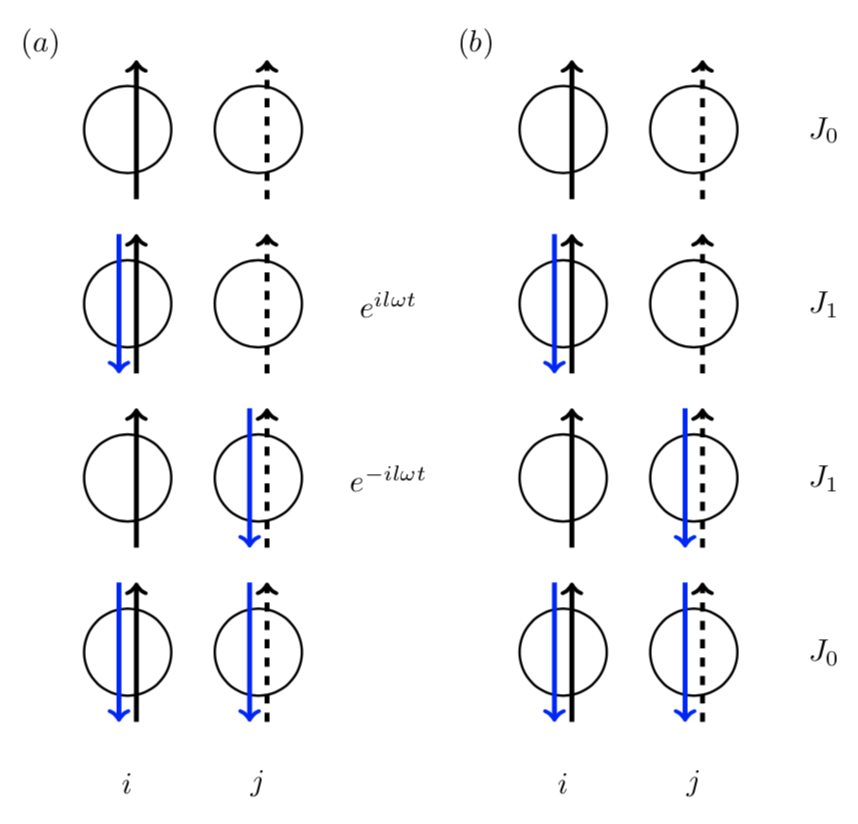
\includegraphics[width=0.8\columnwidth]{chap4_floq/correlated_tunneling_schematic}
\caption{关联隧穿效应示意图:
(a) 近共振驱动使不同的粒子占据情况下的最近邻跃迁获得有效的相位的示意图;
(b) 有效静态哈密顿量中不同的粒子占据情况下获得不同的最近邻跃迁系数的示意图。}
\label{fig:floq:corrtunn}
\end{figure}

由(参考图 \ref{fig:floq:corrtunn} (a))
\begin{align}
& R_l(t)c_{i\uparrow}^{\dagger}c_{j\uparrow}R_l^{-1}(t)\\
=& \exp(\ii\sum_{j}l\omega t\hat{n}_{j\uparrow}\hat{n}_{j\downarrow})
c_{i\uparrow}^{\dagger}c_{j\uparrow}\exp(-\ii\sum_{j}l\omega t\hat{n}_{j\uparrow}\hat{n}_{j\downarrow})\\
=& c_{i\uparrow}^{\dagger}c_{j\uparrow}\exp(\ii\sum_{j'}l\omega t(\hat{n}_{j'\uparrow}+\delta_{ij'}-\delta_{jj'})\hat{n}_{j'\downarrow})\exp(-\ii\sum_{j}l\omega t\hat{n}_{j\uparrow}\hat{n}_{j\downarrow})\\
=& c_{i\uparrow}^{\dagger}c_{j\uparrow} \exp(\ii l\omega t(\hat{n}_{i\downarrow}-\hat{n}_{j\downarrow})) 
\end{align}
和
\begin{align}
\ii\partial_tR_l(t) &= \ii\partial_t \exp(\ii\sum_{j}l\omega t\hat{n}_{j\uparrow}\hat{n}_{j\downarrow}) \\
&= -l \omega \hat{n}_{j\uparrow}\hat{n}_{j\downarrow} R_l(t) 
\end{align}
可得,变换后的哈密顿量为
\begin{align}
\hat{H}(t) =& -J \sum_{\substack{\langle i,j\rangle \\ \sigma = \uparrow,\downarrow}}e^{i\mathbf{d_{ij}}\cdot \tilde{\mathbf{A}}(t)/\hbar} \hat{c}_{i\sigma}^{\dagger}\hat{c}_{j\sigma}+ \tilde{U}\sum_i\hat{n}_{i\uparrow}\hat{n}_{i\downarrow} \label{eq:htt}
\end{align}
其中有效相互作用强度
\begin{align}
\tilde{U}=U-l\hbar\omega
\end{align}
而含时规范势被重整为
\begin{align}
\tilde{\mathbf{A}}_{ij,\sigma}(t)&=\mathbf{A}(t)-\frac{l\omega t}{d^2} \mathbf{d_{ij}}((1-\hat n_{i\bar\sigma})\hat n_{j\bar\sigma}-(1-\hat n_{j\bar\sigma})\hat n_{i\bar\sigma}))
\end{align}
可看出 $\tilde{A}(t)$ 显式地依赖于最近邻粒子数的占据。
在这里显式地看出近共振驱动带来的关联(correlated)效应。


\subsection{近共振驱动下的有效静态模型}
上面的 $R_l(t)$ 只是对含时哈密顿量做了一个幺正变换,体系还是含时的,就已经可以看出规范势的关联效应。这一节推导其有效静态模型,而有效静态模型下关联效应也更加明显。

对于 (\ref{eq:htt}) 式中的哈密顿量 $H(t)$,由于是高频近共振驱动,有 $J, \tilde{U}\ll\hbar\omega$,因此可以对其做高频展开截断以得到有效静态哈密顿量。有效静态哈密顿量的最低阶为 $H(t)$ 的傅立叶零分量,
\begin{align}
H_0 &= -J \sum_{\substack{\langle i,j\rangle \\ \sigma = \uparrow,\downarrow}} \left(\dfrac{1}{T}\int_0^Te^{i\mathbf{d_{ij}}\cdot \tilde{\mathbf{A}}(t)/\hbar}dt\right) \hat{c}_{i\sigma}^{\dagger}\hat{c}_{j\sigma}+ \tilde{U}\sum_i\hat{n}_{i\uparrow}\hat{n}_{i\downarrow} 
\end{align}
利用贝塞尔函数的积分表示 (\ref{eq:bessel}) 式可得,截断到最低阶的有效静态哈密顿量为
\begin{align}
\hat{H}_{\text{eff}} = \sum_{\langle i,j\rangle, \sigma} -\hat{J}^{\langle ij\rangle}_{\text{eff},\sigma}\hat{c}_{i\sigma}^{\dagger}\hat{c}_{j\sigma} + \tilde{U}\sum_{i}\hat{n}_{i\uparrow}\hat{n}_{i\downarrow}
\end{align}
其中
\begin{align}
\hat{J}^{\langle ij\rangle}_{\text{eff},\sigma}=J_0\hat{a}_{ij\bar{\sigma}}+J_1\hat{b}_{ij\bar{\sigma}}
\end{align}
这里有
\begin{align}
J_0 &= JB_0(mA\omega d/\hbar), \\
J_1 &= J B_l(\eta_{ij}mA\omega d/\hbar), \\
\hat{a}_{ij\sigma} &= (1-\hat{n}_{i\sigma})(1-\hat{n}_{j\sigma}) + \hat{n}_{i\sigma}\hat{n}_{j\sigma},\\
\hat{b}_{ij\sigma} &= (-1)^l(1-\hat{n}_{i\sigma})\hat{n}_{j\sigma} + \hat{n}_{i\sigma}(1-\hat{n}_{j\sigma}).
\end{align}
% \begin{align}
% \hat{a}_{ij\sigma} &= (1-\hat{n}_{i\sigma})(1-\hat{n}_{j\sigma}) + \hat{n}_{i\sigma}\hat{n}_{j\sigma},\\
%     \hat{b}_{ij\sigma} &= (-1)^l(1-\hat{n}_{i\sigma})\hat{n}_{j\sigma} + \hat{n}_{i\sigma}(1-\hat{n}_{j\sigma}).
% \end{align}
$\bar{\sigma}$ 表示 $\sigma$ 的补集,而
$\eta_{ij}$ 的定义为,
对于 $(i_x,i_y)=(j_x\pm1,j_y)$ 或是 $(i_x,i_y)=(j_x,j_y\pm 1)$ 的情况有 $\eta_{ij}=\pm 1$。

在如上的有效哈密顿量中,关联隧穿效应显式地体现出来。当调节驱动频率$\omega$ 和驱动振幅 $A$ 使得 $J_0\neq J_1$ 时,最近邻跃迁的过程将显式地依赖于最近邻的一对格点是双占据($J_0$)还是单占据($J_1$)。参考图 \ref{fig:floq:corrtunn} (b) 。对该体系的详细研究还可参考作者与张鹏飞同学\footnote{一只小猪}和翟荟教授的文章\inlinecite{floqhubb}。




\section{关联隧穿效应诱导的铁磁态与相分离} \label{sec:floqhubb}

上一节我们得到了二维正方晶格 Fermi Hubbard 模型在近共振高频驱动下的有效静态哈密顿量,
\begin{align}
\hat{H}_{\text{eff}} &= - \sum_{\langle i,j\rangle, \sigma} 
\left(J_0[(1-\hat{n}_{i\bar\sigma})(1-\hat{n}_{j\bar\sigma}) + \hat{n}_{i\bar\sigma}\hat{n}_{j\bar\sigma}]
+J_1[(-1)^l(1-\hat{n}_{i\bar\sigma})\hat{n}_{j\bar\sigma} + \hat{n}_{i\bar\sigma}(1-\hat{n}_{j\bar\sigma})]\right)
\hat{c}_{i\sigma}^{\dagger}\hat{c}_{j\sigma} \nonumber\\
& \quad + \tilde{U}\sum_{i}\hat{n}_{i\uparrow}\hat{n}_{i\downarrow}
\end{align}
其中第一项为具有关联隧穿效应的动能项,第二项为 Hubbard 相互作用项。式中 $J_0$ 为常数,而 $J_1$ 对于 $\eta_{ij}$ 具有隐含的依赖。事实上,容易验证,当 $l$ 为偶数时,由于贝塞尔偶数阶函数为偶函数,即 $B_l$ 为偶函数,从而此时 $J_1$ 对 $\eta_{ij}$ 依赖是平庸的,在这种情况下 $J_1$ 退化为常数。另一个需要注意到的事实是,当 $l$ 为偶数时
\footnote{该SO(4)对称性由两个SU(2)对称性构成,自旋SU(2)和电荷SU(2),参见第 \ref{sec:so4} 小节。 当 $l$ 为奇数时,容易验证,体系还具有自旋SU(2)对称性,但不再具有电荷自旋SU(2)对称性。}
,模型具有SO(4)对称性(参考第 \ref{sec:so4} 小节),且对于半填充的系统具有粒子空穴对称性。因此,在下面我们着重讨论 $l$ 为偶数的情况。半填充时,模型写作
\begin{align}
\hat{H}_{\text{eff}} &= - \sum_{\langle i,j\rangle, \sigma} 
\left(J_0[(1-\hat{n}_{i\bar\sigma})(1-\hat{n}_{j\bar\sigma}) + \hat{n}_{i\bar\sigma}\hat{n}_{j\bar\sigma}]
+J_1[(-1)^l(1-\hat{n}_{i\bar\sigma})\hat{n}_{j\bar\sigma} + \hat{n}_{i\bar\sigma}(1-\hat{n}_{j\bar\sigma})]\right)
\hat{c}_{i\sigma}^{\dagger}\hat{c}_{j\sigma} \nonumber\\
& \quad + \tilde{U}\sum_{i}\left(\hat{n}_{i\uparrow}-\frac{1}{2}\right)\left(\hat{n}_{i\downarrow}-\frac{1}{2}\right)
\end{align}


\subsection{路径积分平均场方法} \label{sec:floq:pathint}
这里我们采用标准路径积分的方法来推导其平均场哈密顿量。用路径积分的语言,体系的实时配分函数写作
\begin{align}
\mathcal{Z}=&\int \mathcal D\psi D\bar\psi \exp(i\int dt L)  \\
L=&\sum_{i,\sigma} i\bar \psi_{i\sigma}\partial_t\psi_{i\sigma}+\sum_{\langle i,j\rangle, \sigma} \left(J_0a_{ij\bar{\sigma}}(\bar\psi \psi) + J_1b_{ij\bar{\sigma}}^l(\bar\psi\psi)\right)\bar \psi_{i\sigma}\psi_{j\sigma} \notag \\&- \tilde{U}\sum_{i}\bar\psi_{i\uparrow}\psi_{i\uparrow}\bar\psi_{i\downarrow}\psi_{i\downarrow} \  .
\end{align}
这里 $\psi$ 代表费米场算符,$a_{ij\bar{\sigma}}$ 和 $b_{ij\bar{\sigma}}^l$ 是由 $\hat a_{ij\bar{\sigma}}$ 和 $\hat b_{ij\bar{\sigma}}^l$ 替换为场算符。注意到,现在的哈密顿量的动能项是六费米子算符项,传统的基于 Hubbard-Stratonovich 变换的直接解藕得到平均场哈密顿量(那是对于四费米子算符哈密顿量)的方式将不能采用,这里我们采用继承了 Hubbard-Stratonovich 变换的精神的另一种方法。具体来说,对上式路径积分插入 $\delta$-函数来引入辅助玻色场:
\begin{align}
\mathcal{Z}=&\int \mathcal D\psi D\bar\psi Dn \prod_{i\sigma}\delta(n_{i,\sigma}-\bar\psi_{i,\sigma}\psi_{i,\sigma})\exp(i\int dt L)\\
L=&\sum_{i,\sigma} i\bar \psi_{i\sigma}\partial_t\psi_{i\sigma}+\sum_{\langle i,j\rangle, \sigma} \left(J_0a_{ij\bar{\sigma}}(n) + J_1b_{ij\bar{\sigma}}^l(n)\right)\bar \psi_{i\sigma}\psi_{j\sigma}  \notag \\&- \tilde{U}\sum_{i}n_{i\uparrow}n_{i\downarrow} \  .
\end{align}
由于有 $\delta$-函数的存在,上式作用量里的所有 $\bar\psi\psi$ 都可以被替换成 $n$ 场。作为等价性的证明,容易验证,如果将上式中的 $n$ 场先积掉,能够回到原始的路径积分。

现在我们引入另一个 $\eta$ 场来吸收掉作用量中的 $\delta$-函数:
\begin{align}
\mathcal{Z}=&\int \mathcal D\psi D\bar\psi Dn D\eta\exp(i\int dt L)\\
L=&\sum_{i,\sigma} i\bar \psi_{i\sigma}\partial_t\psi_{i\sigma}+\sum_{\langle i,j\rangle, \sigma} \left(J_0a_{ij\bar{\sigma}}(n) + J_1b_{ij\bar{\sigma}}^l(n)\right)\bar \psi_{i\sigma}\psi_{j\sigma}  \notag \\&- \tilde{U}\sum_{i}n_{i\uparrow}n_{i\downarrow}-\sum_{i \sigma}\eta_{i\sigma}(n_{i,\sigma}-\bar\psi_{i,\sigma}\psi_{i,\sigma})
\end{align}
可以看出,这样以来作用量中的费米子场就都变成了二次型。一般来说,我们总可以通过将费米子场积掉来得到有效的玻色场作用量。而平均场近似是说,将这里的玻色场(积分)用其鞍点的值来代替(所以也叫鞍点近似)。由上式做勒让德变换,这就得到平均场哈密顿量,
\begin{align}\label{eq:Hmf0}
    \hat{H} = \sum_{\langle i,j\rangle, \sigma} - \left(J_0a_{ij\bar{\sigma}}(n) + J_1b_{ij\bar{\sigma}}^l(n)\right)\hat{\psi}^{\dagger}_{i\sigma}\hat{\psi}_{j\sigma}  + \tilde{U}\sum_{i}n_{i\uparrow}n_{i\downarrow}+\sum_{i \sigma}\eta_{i\sigma}(n_{i,\sigma}-\hat{\psi}^{\dagger}_{i,\sigma}\hat{\psi}_{i,\sigma}) 
\end{align}
这其中做了如下替换,
 \begin{align}
    \hat{a}_{ij\sigma} &= (1-\hat{n}_{i\sigma})(1-\hat{n}_{j\sigma}) + \hat{n}_{i\sigma}\hat{n}_{j\sigma}, \rightarrow (1-n_{i\sigma})(1-n_{j\sigma}) + n_{i\sigma}n_{j\sigma}\\
    \hat{b}_{ij\sigma} &= (-1)^l(1-\hat{n}_{i\sigma})\hat{n}_{j\sigma} + \hat{n}_{i\sigma}(1-\hat{n}_{j\sigma})\rightarrow (-1)^l(1-n_{i\sigma})n_{j\sigma} + n_{i\sigma}(1-n_{j\sigma})
 \end{align}

对于半填充、自旋平衡的体系,注意到这时费米面嵌套效应的存在(沿$(\pi,\pi)$方向),对于通常的 Fermi Hubbard 模型,无穷小相互作用就可以引发体系的序($(\pi,\pi)$ 自旋密度波或电荷密度波或超导配对)。同时注意到,$l$ 为偶数的情况系统具有SO(4)对称性,因此电荷密度波序与超导配对的序简并\cite{yang1990},而自旋密度波的三个方向($s_z$, $s_x$, $s_y$)也简并\cite{yang1990}。因此可将序参量取在电荷密度波方向(吸引相互作用),或自旋密度波$z$方向(排斥相互作用)\cite{floqhubb}。

现在将局域格点上的粒子数密度用电荷密度波序与自旋密度波序来表示,
\begin{align}
    n_{i\uparrow} = \frac{1}{2}(1 + c_i + s_i ) \;,\;\; n_{i\downarrow} = \frac{1}{2}(1+c_i-s_i)
\end{align}
这里 $c$ 和 $s$ 分别是电荷密度波(Charge Density Wave, CDW)序参量和自旋密度波(Spin Density Wave, SDW)序参量。

我们现在关注两种情况。
\begin{enumerate}
    \item $c_i=(-1)^{i_x+i_y}c$, $s_i=(-1)^{i_x+i_y}s$
    \item $c_i=(-1)^{\lceil i_x/L \rceil + \lceil i_y/L \rceil}c, s_i=(-1)^{\lceil i_x/L \rceil + \lceil i_y/L \rceil}s$  
\end{enumerate}
这里 $\lceil x \rceil$ 表示关于 $x$ 的天花板函数,即向上取整函数。将两式分别带入(\ref{eq:Hmf0})式,可以得到两种情况下的平均场哈密顿量。

\begin{figure}[!htb]
\centering
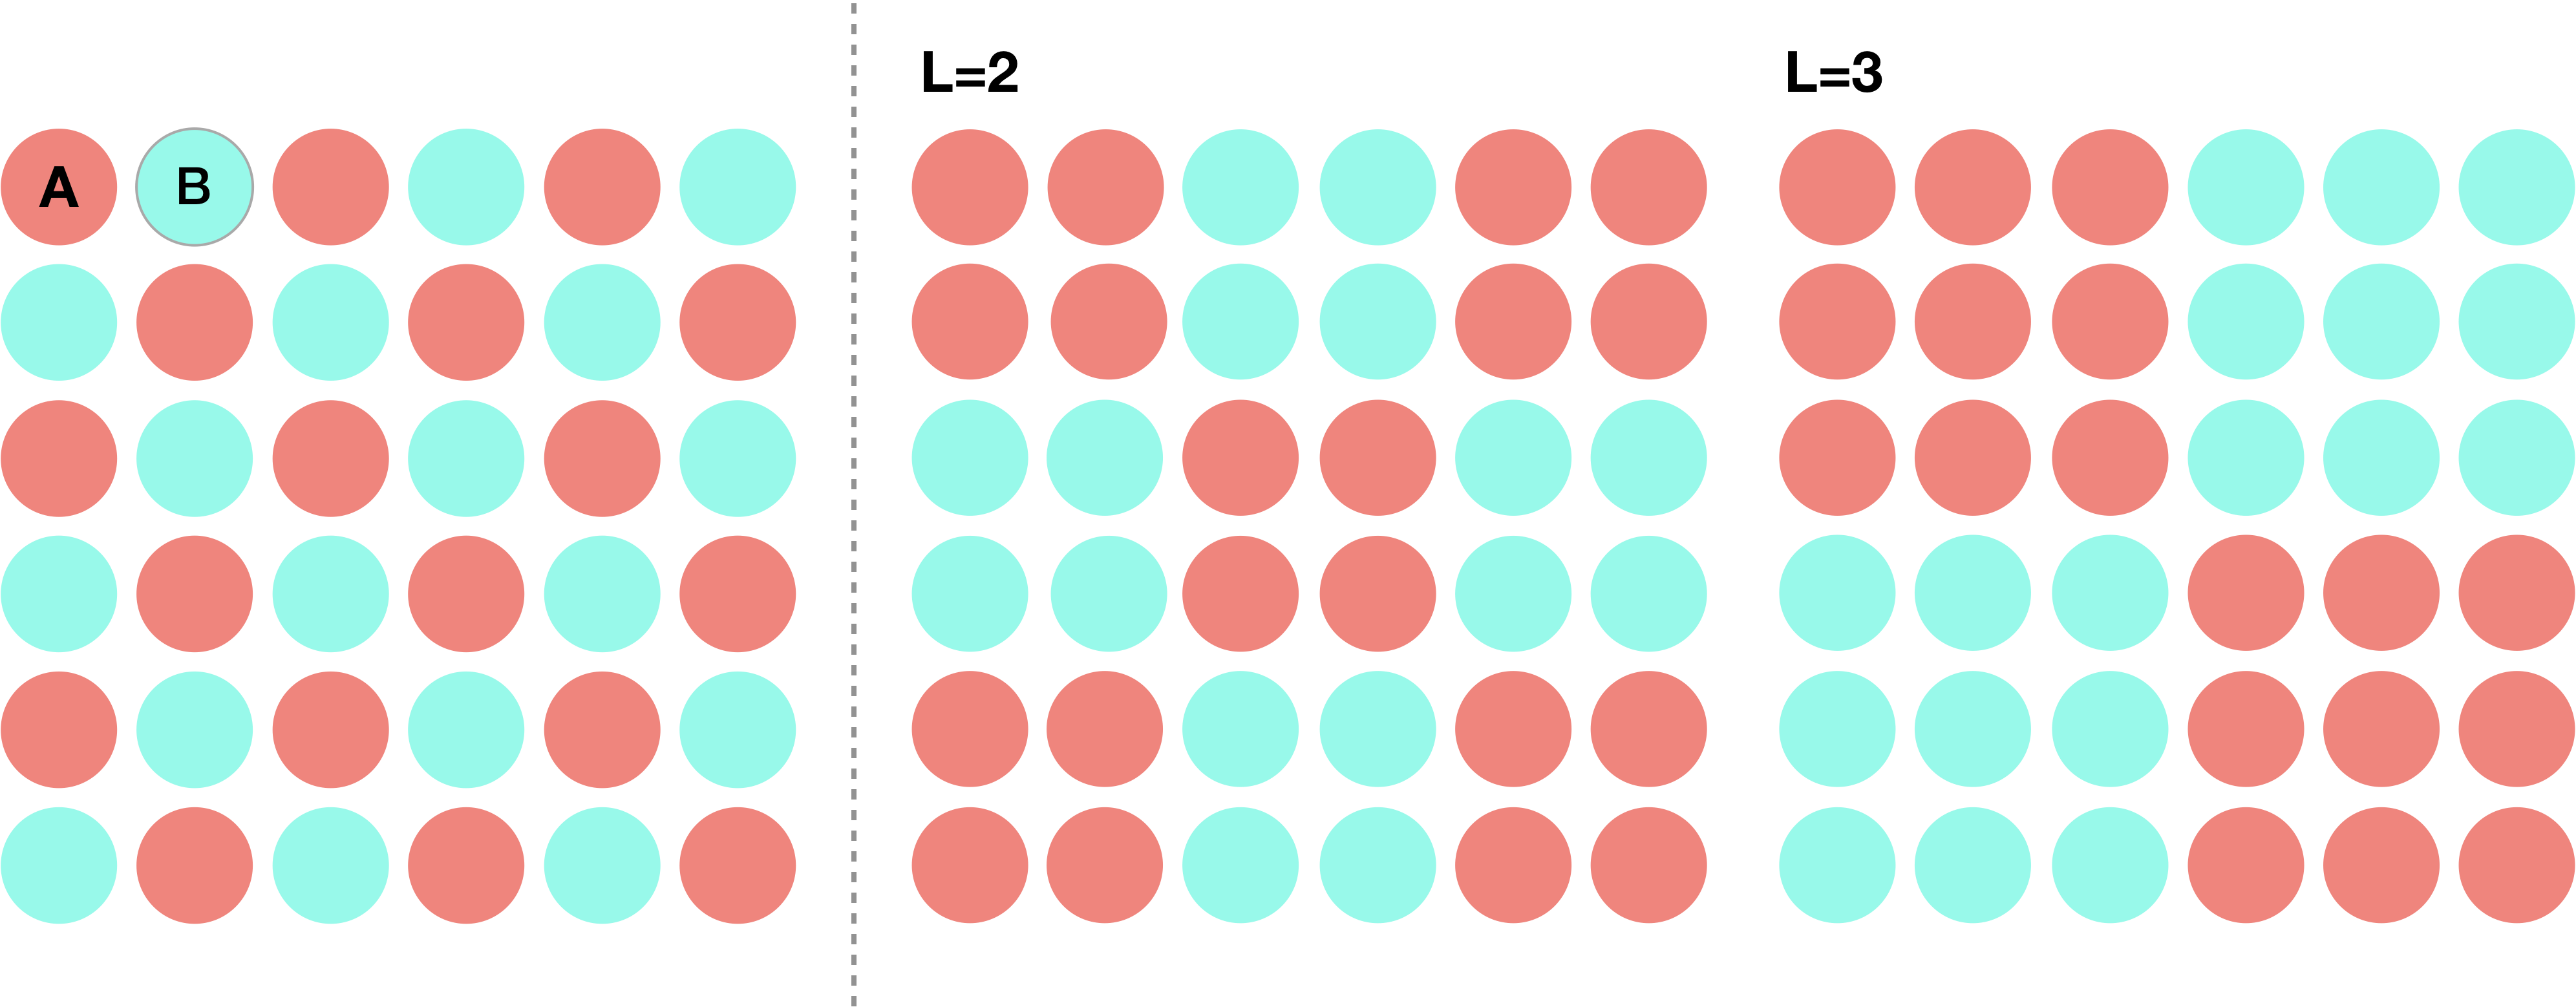
\includegraphics[width=1.0\columnwidth]{chap4_floq/cdwsdw}
\caption{电荷(自旋)密度波示意图。左:第一种情况,即 $(\pi,\pi)$ 序参量的情况。右:第二种情况,即元胞扩大化的情况。这里以 $L=2$ 和 $L=3$ 为例。}\label{fig:floq:cdwsdw}
\end{figure}

第一种情况为 $(\pi,\pi)$ 序参量\cite{nagaosa},这时晶格被自然地划分为 $A/B$ 两套子晶格,见图 \ref{fig:floq:cdwsdw} (左) 示意图。第二种情况为 $(\pi/L,\pi/L)$ 的序参量,也就是元胞扩大化的情况,见图 \ref{fig:floq:cdwsdw} (右) $L=2$ 和 $L=3$ 的示意图。


\subsection{平均场基态的自洽求解}
对上一小节得到的平均场哈密顿量,数值求解自洽解即可得到其平均场基态。这里,我们对第一种情况进行详细的说明计算流程。对第一种情况,此时有
\begin{align}
    &n_A\equiv\langle \hat{n}_{i\in A} \rangle = 1 + c , \  \  \
    s_A\equiv\langle \hat{S}_{i\in A}^{z} \rangle = s/2,\label{order1} \\
    &n_B\equiv\langle \hat{n}_{i\in B} \rangle = 1 - c , \  \  \
    s_B\equiv\langle \hat{S}_{i\in B}^{z} \rangle = -s/2,\label{order2}
\end{align}
带入(\ref{eq:Hmf0})式,平均场哈密顿量显式地写为,
\begin{align}\label{eq:Hmf}
    \hat{H}_{\text{mf}} &= \sum_{\langle i,j\rangle,\sigma} \left\{-J_0[(1-n_{A\bar{\sigma}})(1-n_{B\bar{\sigma}})+n_{A\bar{\sigma}}n_{B\bar{\sigma}}] - J_1[(1-n_{A\bar{\sigma}})n_{B\bar{\sigma}}+n_{A\bar{\sigma}}(1-n_{B\bar{\sigma}})]\right\}\hat{c}_{i\sigma}^{A\dagger}\hat{c}_{j\sigma}^B+ \text{H. C. } \notag \\
    & \  \  + \eta_c \left[c-\frac{(\hat{n}_{A\uparrow}+\hat{n}_{A\downarrow}) - (\hat{n}_{B\uparrow}+\hat{n}_{B\downarrow})}{2}\right] 
    + \eta_s \left[s-\frac{(\hat{n}_{A\uparrow}-\hat{n}_{A\downarrow}) - (\hat{n}_{B\uparrow}-\hat{n}_{B\downarrow})}{2}\right] \notag \\
    & \  \  + \frac{\tilde{U}N}{2}(n_{A\uparrow}n_{A\downarrow} + n_{B\uparrow}n_{B\downarrow}) 
\end{align}
其中 $\hat{c}_{i\sigma}^A$($\hat{c}_{i\sigma}^B$) 是第 $i$ 个元胞属于 $A(B)$ 子格的自旋为 $\sigma$ 的费米子湮灭算符。$\hat{n}_{\mu\sigma} = \frac{1}{N/2}\sum_{i\in\mu}\hat{n}_{i\sigma}$, $\mu = A$ or $B$ 而 $n_{\mu\sigma} = \langle\hat{n}_{\mu\sigma}\rangle$。$\eta_c$ 和 $\eta_s$ 分别是 CDW 和 SDW 的拉格朗日乘子,同样也是最小化得到基态能量的变分序参量之一。

将以上平均场哈密顿量变换到动量空间,写作
\begin{align}\label{eq:Hmfk}
    \hat{H}_{\text{mf}} &= \sum_{\mathbf{k}\sigma}-P_{\sigma}(c,s)Q(\mathbf{k})\hat{c}_{\mathbf{k}\sigma}^{A\dagger}\hat{c}_{\mathbf{k}\sigma}^B+ \text{H.c.} 
        + \frac{\tilde{U}N}{2}(1+c^2-s^2) \notag\\
        & \  \  \ 
        + \eta_c \left[c-\frac{(\hat{n}_{A\uparrow}+\hat{n}_{A\downarrow}) - (\hat{n}_{B\uparrow}+\hat{n}_{B\downarrow})}{2}\right]
        + \eta_s \left[s-\frac{(\hat{n}_{A\uparrow}-\hat{n}_{A\downarrow}) - (\hat{n}_{B\uparrow}-\hat{n}_{B\downarrow})}{2}\right]
\end{align}
其中 $\hat{c}_{\mathbf{k}\sigma}^A$($\hat{c}_{\mathbf{k}\sigma}^B$) 是 $A(B)$ 子格准动量为 $\mathbf{k}$ 的费米子湮灭算符,$Q(\mathbf{k}) = \sum_{i}\exp(i\mathbf{k}\cdot\mathbf{d}_i)$,$\{\mathbf{d}_i\}$ 是晶格矢量,而
\begin{align}
    P_{\uparrow}(c,s) &= \frac{J_0}{2}\left[1-(c-s)^2\right] + \frac{J_1}{2}\left[1+(c-s)^2\right] \\
    P_{\downarrow}(c,s) &= \frac{J_0}{2}\left[1-(c+s)^2\right] + \frac{J_1}{2}\left[1+(c+s)^2\right] 
\end{align} 
式 (\ref{eq:Hmfk}) 中求和 $\vecr{k}$ 的空间为第一布里渊区。通过对 (\ref{eq:Hmfk}) 式哈密顿量进行变分求极值,即可得到平均场基态解。

这里需要说明的是,Feynman-Hellman 定理告诉我们
\begin{align}
\langle\partial H(\lambda)/\partial \lambda\rangle=\partial E(\lambda)/\partial \lambda
\end{align}
那么对于 (\ref{eq:Hmfk})式哈密顿量求多体基态,相当于去找(基态)能量的极值,也即
\begin{align}
\partial E(para.)/\partial para. =0
\end{align}
$para.$ 代表哈密顿量中的变分参数。利用 Feynman-Hellman 定理得,
\begin{align}\label{eq:selfconsist}
    \sum_{k,i} u^*_i(k)\dfrac{\partial\mathcal{H}(k;para.)}{\partial para.}u_i(k)\Theta(-\epsilon_i(k))+\dfrac{\partial const.}{\partial para.}=0 
\end{align} 
也就是去找以上方程(组)的自洽解(或者说,找等式左边的零点)。

现在我们对 (\ref{eq:Hmfk}) 式哈密顿量进行这样的计算。$\hat{H}_{\text{mf}}$ 中各项对各个变分参数的偏导如下。
令 $const.$ 表示常数部分\footnote{相当于常数$\times$单位矩阵},
即 
\begin{align}
const. = \frac{\tilde{U}N}{2}(1+c^2-s^2) + \eta_cc+\eta_ss
\end{align}
因此有
\begin{align}
\dfrac{\partial const.}{\partial c} &= \tilde{U}Nc+\eta_c \\
\dfrac{\partial const.}{\partial s} &= -\tilde{U}Ns+\eta_s \\
\dfrac{\partial const.}{\partial \eta_c} &= c \\
\dfrac{\partial const.}{\partial \eta_s} &= s 
\end{align}
令 $\mathcal{H}(k)$ 表示矩阵部分,有
\begin{align}
    & \dfrac{\partial\mathcal{H}(k)}{\partial c}=
        \begin{pmatrix}
            0 & -\frac{\partial P_{\uparrow}}{\partial c}Q(k) & & \\
            -\frac{\partial P_{\uparrow}}{\partial c}Q(-k) & 0 & & \\
            & & 0 & \frac{\partial P_{\downarrow}}{\partial c}Q(k) \\
            & & \frac{\partial P_{\downarrow}}{\partial c}Q(-k) & 0 
        \end{pmatrix}
\end{align}
\begin{align}
    & \dfrac{\partial\mathcal{H}(k)}{\partial s}=
        \begin{pmatrix}
            0 & -\frac{\partial P_{\uparrow}}{\partial s}Q(k) & & \\
            -\frac{\partial P_{\uparrow}}{\partial s}Q(-k) & 0 & & \\
            & & 0 & \frac{\partial P_{\downarrow}}{\partial s}Q(k) \\
            & & \frac{\partial P_{\downarrow}}{\partial s}Q(-k) & 0 
        \end{pmatrix}
\end{align}
\begin{align}
    & \dfrac{\partial\mathcal{H}(k)}{\partial \eta_c}=\dfrac{1}{2}
        \begin{pmatrix}
            -1 & & & \\
            & 1 & & \\
            & & 1 & \\
            & & & -1 
        \end{pmatrix}
\end{align}
\begin{align}
    & \dfrac{\partial\mathcal{H}(k)}{\partial \eta_s}=\dfrac{1}{2}
        \begin{pmatrix}
            -1 & & & \\
            & 1 & & \\
            & & -1 & \\
            & & & 1 
        \end{pmatrix} 
\end{align}
其中,
\begin{align}
    \dfrac{\partial P_{\uparrow}}{\partial c} 
        &= (J_1-J_0)(c-s) = -\dfrac{\partial P_{\uparrow}}{\partial s} \\
    \dfrac{\partial P_{\downarrow}}{\partial c} &= (J_1-J_0)(c+s) = \dfrac{\partial P_{\downarrow}}{\partial s} 
\end{align}


将以上计算结果带入 (\ref{eq:selfconsist}) 式左边,求其零点,即可得平均场基态自洽解。对于 $J_0=J_1$ 的情况,体系回到通常的 Fermi Hubbard 模型。上述平均场哈密顿量回到人们通常用到的形式。注意到,此时对 $c$ 和 $s$ 的变分给出
\begin{align}
\eta_c &= -\tilde{U}Nc \\
\eta_s &= \tilde{U}Ns
\end{align}



\subsection{平均场相图}

\begin{figure}[!htb]
\centering
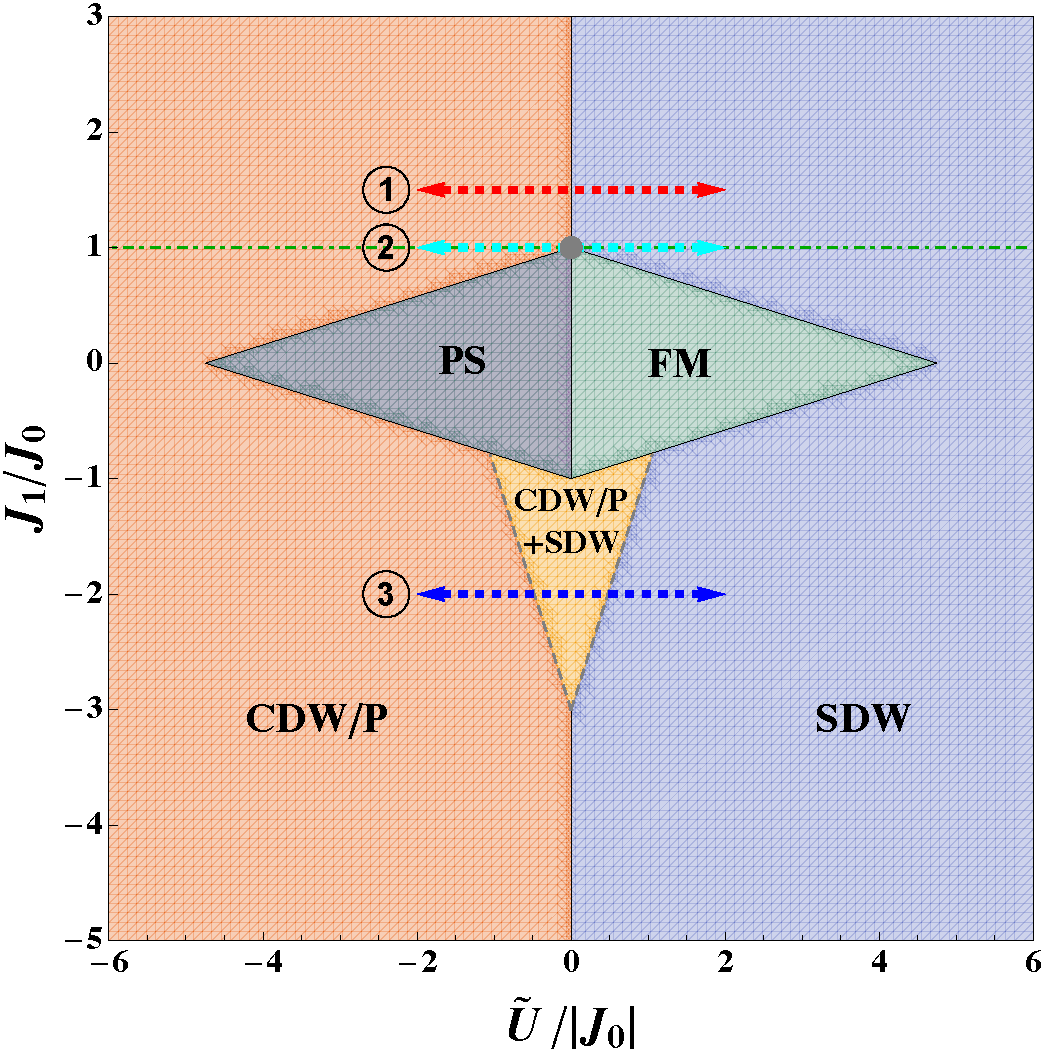
\includegraphics[width=0.9\columnwidth]{floqhubb/Phase_diagram}
\caption{平均场相图。CDW 代表电荷密度波序,SDW 代表自旋密度波序,P 代表费米子库玻配对序(Cooper Pair),PS 代表相分离(Phase Separation),FM 代表铁磁序(Ferromagnetism)。由于SO(4)对称性的存在,CDW 与 P 简并,SDW 三个不同方向简并。CDW/P+SDW 表示 二者共存的相。对于相边界,实线表示一级相变,虚线表示二级相变。$J_1/J_0=1$ 的水平线(绿色点划线)上,体系回到通常的 Fermi Hubbard 模型,这种情况下,由于半填充时费米面的嵌套效应,调节相互作用从吸引到排斥(或从排斥到吸引)的相变为二级相变,图中以灰色粗点标出。1(红),2(青),3(蓝)这三条双向箭头标记图 \ref{fig:floqhubb:orderparameter} 中计算序参量的三种情况。(取自\inlinecite{floqhubb})}
\label{fig:floqhubb:phasediagram}
\end{figure}

根据上一小节的推导,利用计算机程序进行迭代求解可得到平均场基态的自洽解。得到平均场相图如图 \ref{fig:floqhubb:phasediagram}。
% 事实上,由于模型具有 $(J_0, J_1)\leftrightarrow (-J_0, -J_1)$ 的对称性,我们总可以将 $J_0$ 取在 $J_0\geq0$ \cite{floqhubb}。
从相图上可以看到,在大吸引相互作用($\tilde{U}/J_0\ll0$)的区域,体系的基态具有电荷密度波序或超导配对序,而在大排斥相互作用($\tilde{U}/J_0\gg0$)的区域,体系的基态具有自旋密度波序。二者之间的过渡,比较普遍的情况下是一级相变(图 \ref{fig:floqhubb:phasediagram} 中实线相边界),或者经历相共存区域(图 \ref{fig:floqhubb:phasediagram} 中 CDW/P+SDW 区域)。只有在特殊情况下,例如 $J_0=J_1$ 的情况下,二者的过渡是二级相变。这是由于,当 $J_0=J_1$ 时,体系回到通常的 Fermi Hubbard 模型,而二维正方晶格上的 Fermi Hubbard 模型在半填充时费米面具有嵌套的效果,无穷小相互作用就可以引发序的产生,因此 $\tilde{U}\neq0$ 时体系有有序的解,但 $\tilde{U}=0$ 时模型是自由的,显然没有序,因此其相变为二级相变。
\footnote{作为对比,如果是一级相变的话,$\tilde{U}=0$ 应该有两个能量相同的解。参见
图 \ref{fig:floqhubb:phasediagram} 中 1号红色双向箭头,图 \ref{fig:floqhubb:orderparameter} 中间曲线,与
图 \ref{fig:floqhubb:kinetic} 中蓝色实线的行为。}

\begin{figure}[t]
\centering
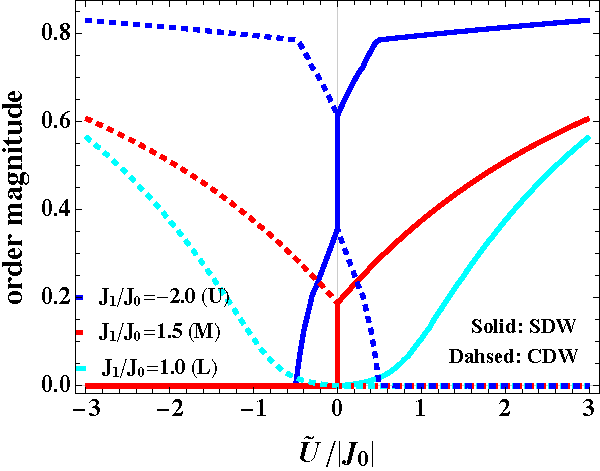
\includegraphics[width=0.9\columnwidth]{floqhubb/order_parameter}
\caption{对于图 \ref{fig:floqhubb:phasediagram} 中三条双向箭头标记曲线上序参量的计算。三种情况分别对应于:(1,中,M,红色)$J_1/J_0=1.5$;(2,下,L,青色)$J_1/J_0=1.0$;(3,上,U,蓝色)$J_1/J_0=-2.0$。其中实线表示 SDW 的序参量曲线,虚线表示 CDW 的序参量曲线。可以看到,中间的红色曲线实线和虚线部分的值在 $\tilde{U}=0$ 处均出现有限大的跳变,代表这种情况下是一级相变。下面的青色曲线的值在 $\tilde{U}=0$ 处连续过渡到 0,代表这是二级相变,这种情况也对应着通常的 Fermi Hubbard 模型,由于半填充时费米面嵌套效应的存在,无限小的相互作用就可以诱导体系出现序\cite{nagaosa}。上面的蓝色曲线中出现以 $\tilde{U}=0$ 为中心的一段 CDW(虚线) 和 SDW(实线)序参量值均不为0的区域,代表这里是 CDW+SDW 的共存相。(取自\inlinecite{floqhubb})}
\label{fig:floqhubb:orderparameter}
\end{figure}

对于一级相变、二级相变、和相共存的情况,我们分别给出三个代表性例子,分别取 $J_1/J_0=1.5$, $J_1/J_0=1.0$, $J_1/J_0=-2.0$,画出序参量的值随 $\tilde{U}/J_0$ 变化的情况,见图 \ref{fig:floqhubb:orderparameter} 三种颜色的曲线,以及图 \ref{fig:floqhubb:phasediagram} 中对应颜色的双向箭头。 具体来说,$J_1/J_0=1.5$ 对应一级相变的情况,见图 \ref{fig:floqhubb:phasediagram} 1号红色双向箭头标示,以及图 \ref{fig:floqhubb:orderparameter} 中间红色曲线的行为;$J_1/J_0=1.0$ 对应二级相变的情况,见图 \ref{fig:floqhubb:phasediagram} 2号青色双向箭头标示,以及图 \ref{fig:floqhubb:orderparameter} 下面青色曲线的行为;$J_1/J_0=-2.0$ 对应穿过相共存区域的情况,见图 \ref{fig:floqhubb:phasediagram} 3号蓝色双向箭头标示,以及图 \ref{fig:floqhubb:orderparameter} 中间蓝色曲线的行为。


相图中最新奇的部分在于中间的铁磁相(FM)和相分离(PS)区域。通过图 \ref{fig:floqhubb:phasediagram} 可看出,铁磁相和相分离发生在小相互作用$\tilde{U}/J_0\lesssim1$、且 $J_1<J_0$ 的区域。引起这两个新奇的相的机制值得探讨。


\subsection{关联隧穿引发铁磁相与相分离的机制}
在图 \ref{fig:floqhubb:phasediagram} 的平均场相图中,在小相互作用,小 $J_1$ 区域出现了铁磁相和相分离结构。对于这两个新奇的相,我们从几种角度来理解其出现的机制。

\begin{figure}[t]
\centering
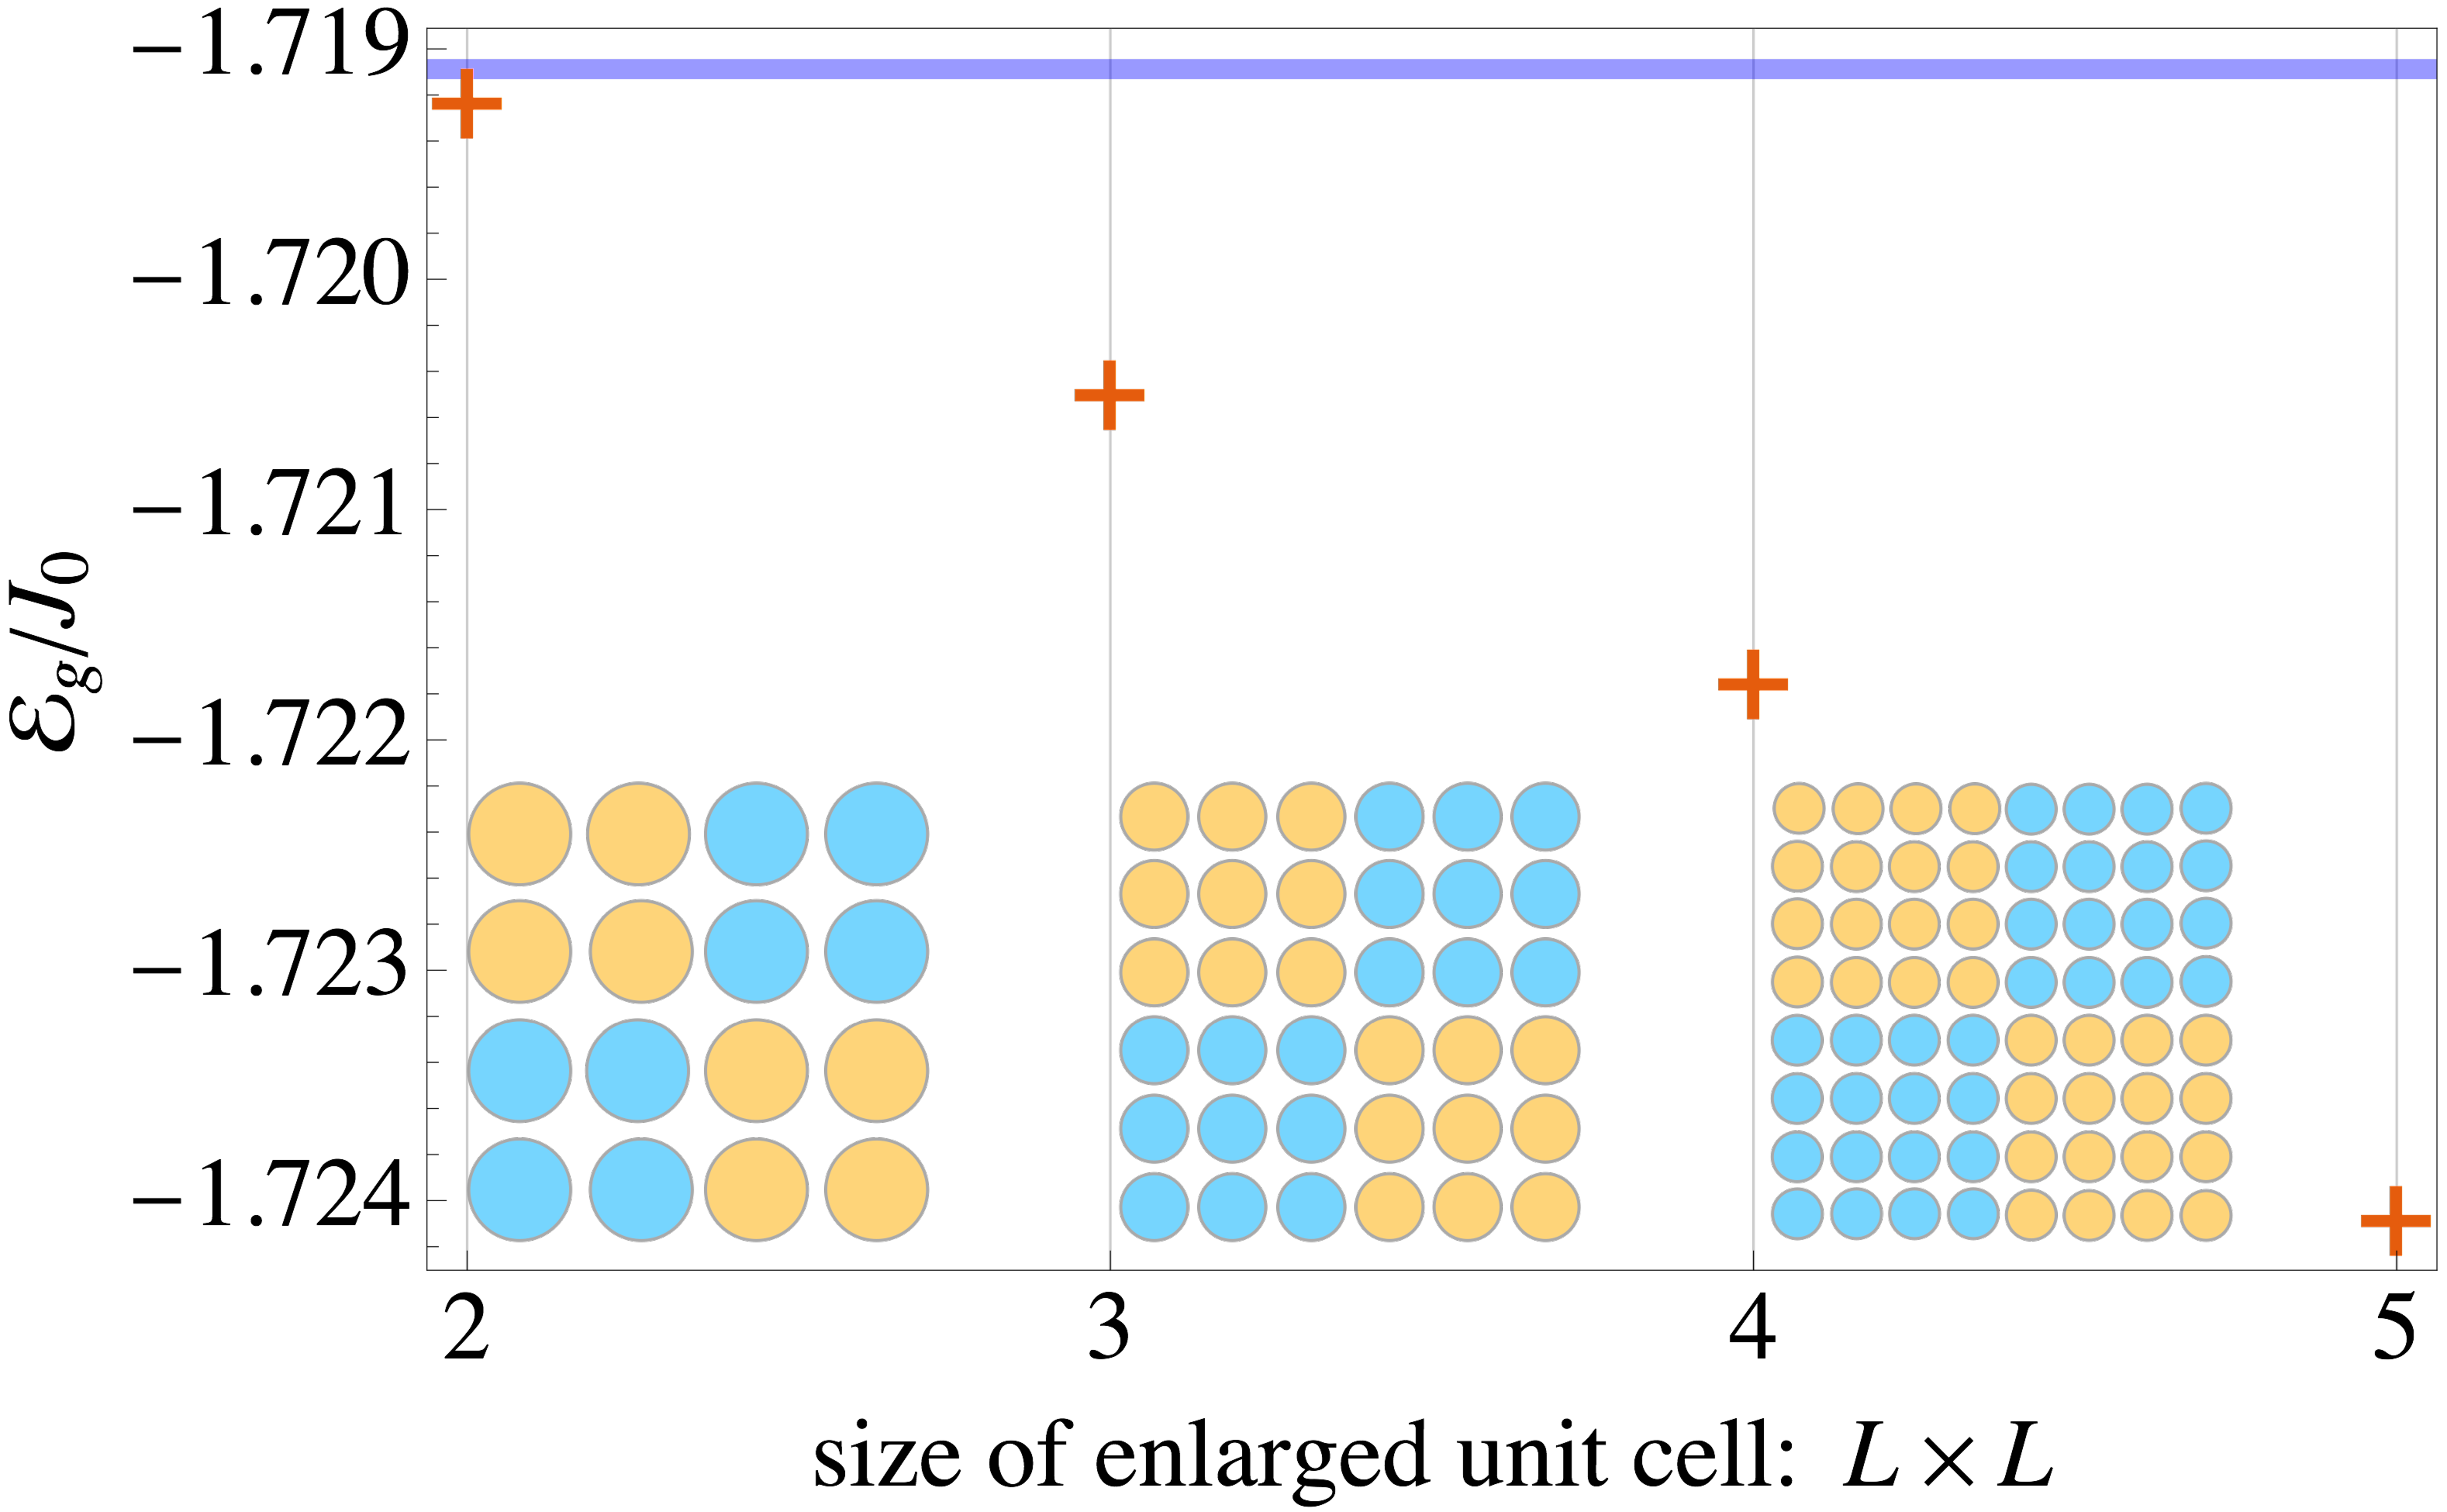
\includegraphics[width=0.9\columnwidth]{floqhubb/phase_seperation}
\caption{平均场基态能量随元胞扩大化参数 $L$ 的变化。对于铁磁相和相分离区域,我们这里取一组代表性的参数,$J_1=0$, $\tilde{U}/|J_0|=-0.2$,数值迭代求解自洽方程组(\ref{eq:selfconsist}),得到元胞扩大化到$L=2,3,4,5$时的平均场基态能量。蓝色的水平线为自由(序参量为0)情况下的能量,$L=1$时只有该自由解。可见随着 $L$ 增大,平均场基态能量单调下降,体系趋向于形成大的磁畴或密度畴(domain)——即铁磁态(排斥相互作用)或相分离(吸音相互作用)。(取自\inlinecite{floqhubb})}
\label{fig:floqhubb:seperation}
\end{figure}

首先,对平均场自洽方程组(\ref{eq:selfconsist})的数值求解显示出铁磁相和相分离。如图 \ref{fig:floqhubb:seperation} 所示,在铁磁相和相分离的区域中,对 \ref{sec:floq:pathint} 节中的元胞扩大化(情况二)的数值迭代求解显示,体系的基态能量随着元胞扩大化的 $L$ 的增大而单调降低。这也就意味着,体系趋向于越来越大的 $L$,最终会形成磁畴和密度畴\footnote{畴,domain}。对于排斥相互作用的情况,即 $\tilde{U}>0$ 时,$c=0$,而$s\neq0$,体系会形成自旋密度波的畴,也就是铁磁态;而对于吸引相互作用的情况,即 $\tilde{U}<0$,$s=0$,而 $c\neq=0$,体系会形成电荷密度波的畴,也就是相分离。
\footnote{参见图 \ref{fig:floq:cdwsdw}(右)示意图,形成自旋密度波磁畴时,相同(不同)颜色的区域具有相同(不同)的 $s_{\uparrow}-s_{\downarrow}$,而形成电荷密度波密度畴时,则为 $n=n_{\uparrow}+n_{\downarrow}$。}

\begin{figure}[t]
\centering
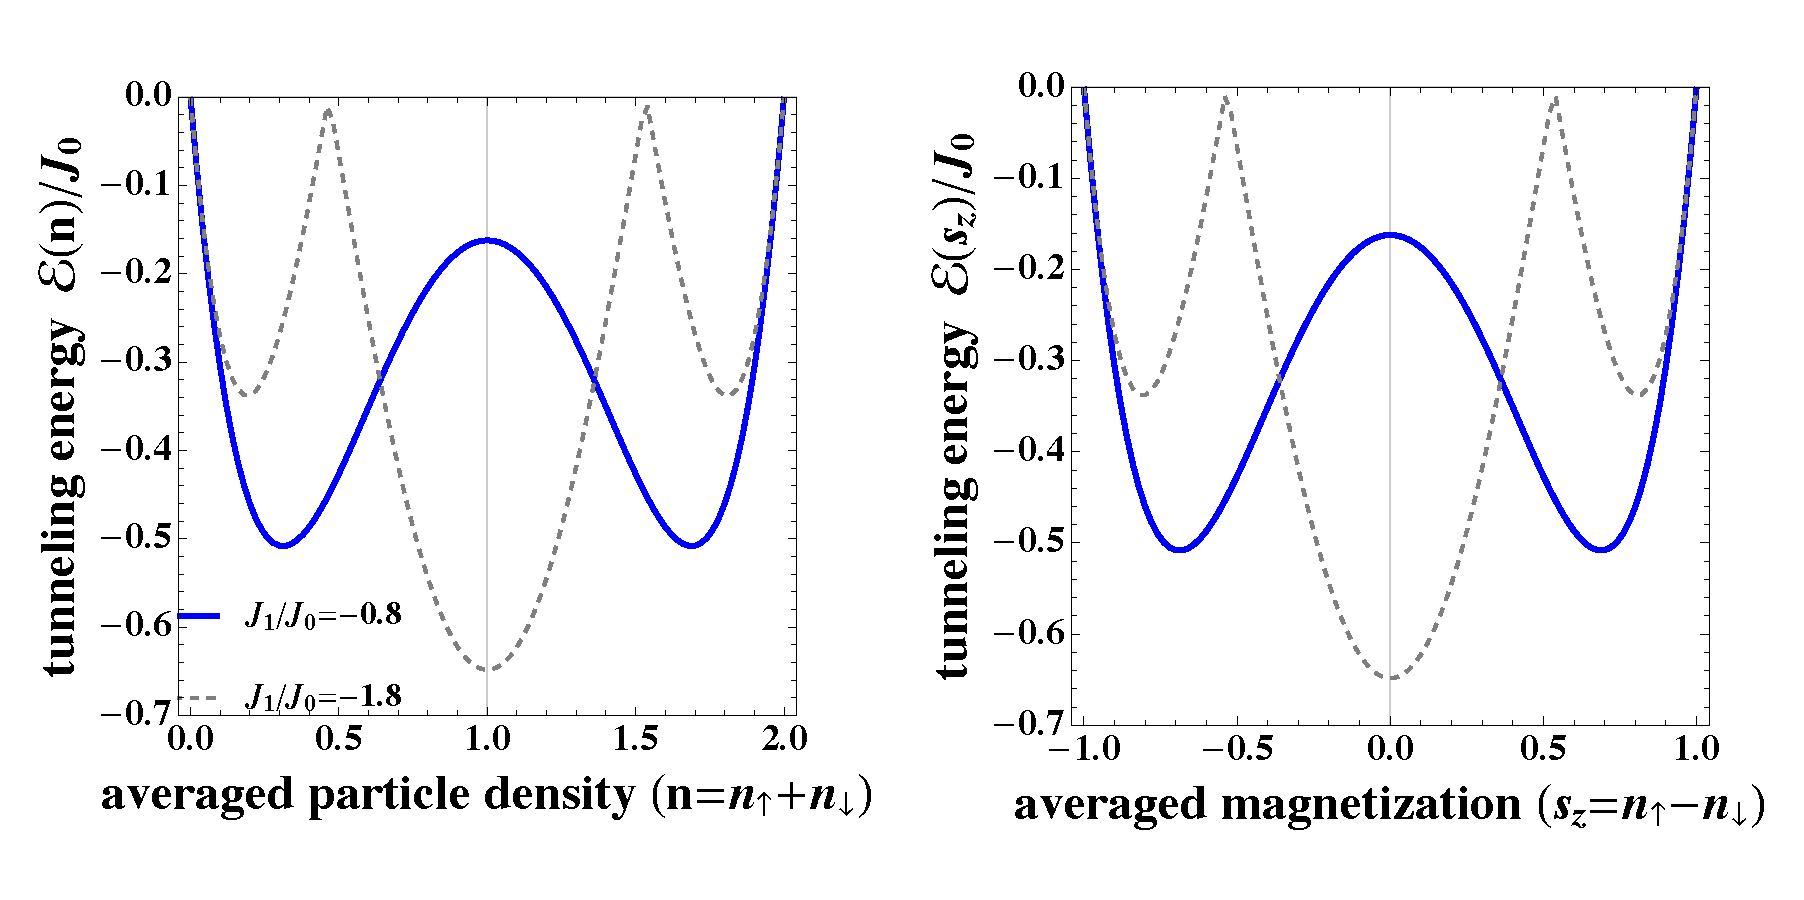
\includegraphics[width=1.\columnwidth]{floqhubb/kinetic_energy}
\caption{$\tilde{U}=0$ 时体系能量作为平均粒子密度密度(左)或平均自旋密度(右)的函数行为。此时,由于相互作用为0,体系的能量等于其跃迁动能。蓝色实现为 $J_1/J_0=-0.8$ 时的情况,此时体系基态能量在左右各有一个极小值点,中间的点为极大值点,是不稳定平衡点,该点位于相图 \ref{fig:floqhubb:phasediagram} PS$\leftrightarrow$FM相变边界上。灰色虚线为 $J_1/J_0=-1.8$ 时的情况,可见体系基态能量在中间有一个最小值,是稳定平衡点,该点位于相图 \ref{fig:floqhubb:phasediagram} 中 CDW$\leftrightarrow$SDW相变边界上。(取自\inlinecite{floqhubb})}
\label{fig:floqhubb:kinetic}
\end{figure}


事实上,这里的铁磁相和相分离的出现是由于哈密顿量动能相中的关联隧穿效应,这可以从如下事实看出。我们考虑元胞扩大化后,畴的内部和相临的畴之间的跃迁系数:
\footnote{也就是图 \ref{fig:floq:cdwsdw}中相同颜色内,与相临的不同颜色之间}
\begin{align}
    J^{\text{intra}}_{\text{eff},\sigma} &= \frac{1}{2} \left(J_0[1+(c\mp s)^2]+J_1[1-(c\mp s)^2]\right), \\
    J^{\text{inter}}_{\text{eff},\sigma} &= \frac{1}{2} \left(J_0[1-(c\mp s)^2]+J_1[1+(c\mp s)^2]\right),
\end{align}
这里 $J^{\text{intra}}_{\text{eff},\sigma}$ 表示畴内$\sigma$-自旋的跃迁系数,而 $J^{\text{inter}}_{\text{eff},\sigma}$ 表示相临畴之间的$\sigma$-自旋的跃迁系数。可以看出,$|J_1|<|J_0|$ 时,$|J^{\text{intra}}_{\text{eff},\sigma}|$ 一直大于 $|J^{\text{inter}}_{\text{eff},\sigma}|$,$|J^{\text{intra}}_{\text{eff},\sigma}|\geq|J^{\text{inter}}_{\text{eff},\sigma}|$ 恒成立,即畴内跃迁系数较畴跃迁系数更大。当相互作用 $\tilde{U}$ 较小时,体系的行为主要有跃迁项主导,而由于畴内跃迁系数较畴间跃迁系数更大,体系倾向于形成大的元胞,以增加畴内跃迁,减少畴间跃迁。


作为一种极限情况,我们来考虑没有相互作用时的情况。此时 $\tilde{U}=0$,模型完全有第一项动能项主导。之前的数值迭代求解都约束在半填充、自旋平衡的情况下来做,这里我们放开这两个约束,计算出体系能量(动能)根据平均粒子数密度 $n$ 和 平均自旋密度 $s$ 变化的行为,见图 \ref{fig:floqhubb:kinetic}。由图 \ref{fig:floqhubb:kinetic} 可见,$|J_1|>|J_0|$ 时,体系基态能量在 $n=1$ 或 $s=0$ 处均为一个极小值点,而 $|J_1|<|J_0|$ 时,体系基态能量在 $n=1$ 或 $s=0$ 处均为一个极大值点,而在其两侧有两个对称的极小值点。这也就说明,当体系加一点微扰相互作用时,后者倾向于落在左右两个极小值点上,形成具有不同电荷密度或自旋密度的畴。这从另一个角度解释了铁磁相和相分离结构的行为。


从以上的分析可以看出,这里的铁磁相和相分离的出现是由于哈密顿量动能项中的关联隧穿效应,且发生于有效相互作用很小的区域,有别于传统 Stoner 机制中由较大相互作用诱发的铁磁。而关联隧穿效应则来自于近共振的高频驱动。因此这种新奇的铁磁相和相分离的产生机制其实是近共振的高频驱动。需要说明的是,由于我们所关注的物理集中在较小相互作用区域,由于费米面的嵌套效应,使得平均场近似的方法相对可靠。而且,鉴于实验上已经实现了类似的哈密顿量\cite{correlated-tunnel-expr-2018-shaking},这样的铁磁相可以期待实验检验。事实上,通过调节驱动频率 $\omega$ 和 振幅 $A$,有多种不唯一的方式来实现相图中的 $\tilde{U}/|J_0|\lesssim1$,$|J_1/J_0|<1$ 的区域。







